\documentclass{article}
\usepackage[paperheight=11in,paperwidth=8.5in,margin=1in]{geometry}
\usepackage{fancyhdr}
\usepackage{graphicx}
\setlength{\headheight}{15.2pt}
\pagestyle{fancy}

\begin{document}
\fancyhf{}
\lhead{Security Crawler}
\chead{MILESTONE 2}
\rhead{\today}

\begin{figure}[h]
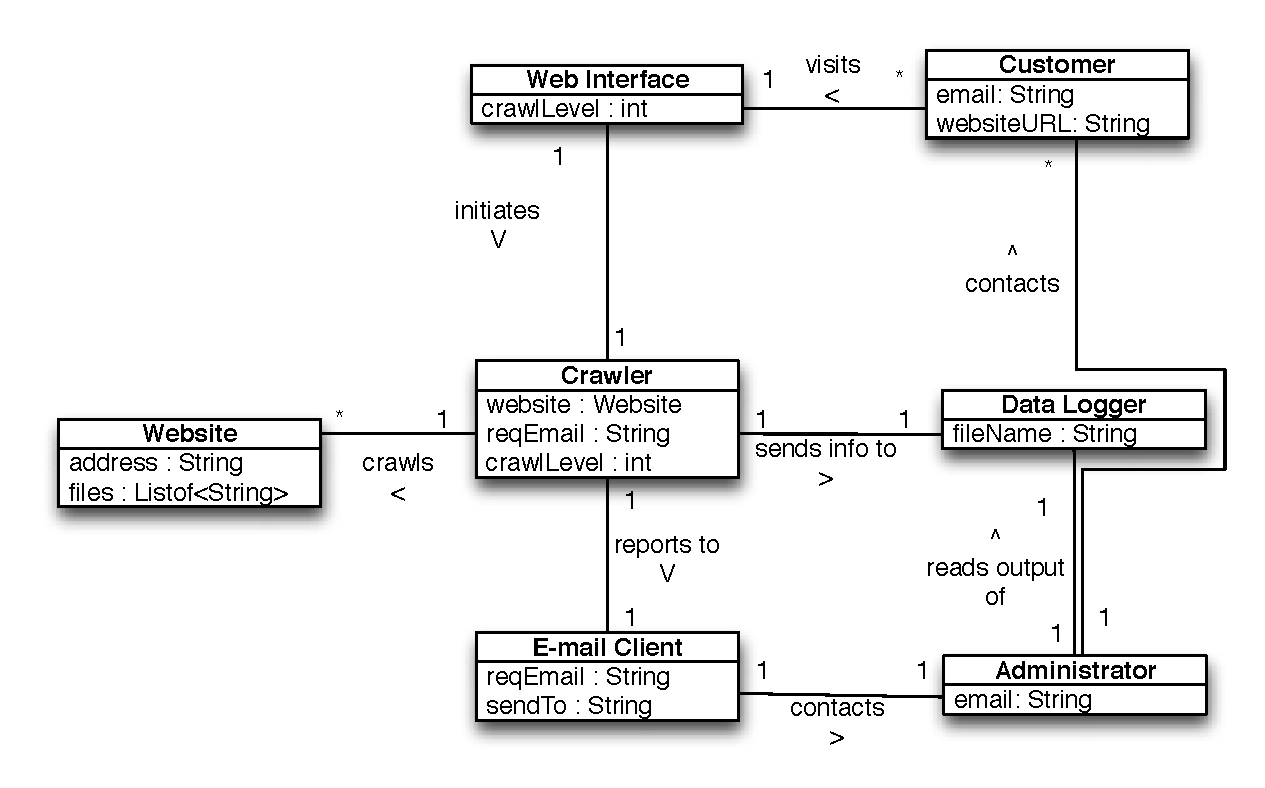
\includegraphics[width=.9\textwidth]{374DM}
\caption{Domain Model}
\end{figure}

\begin{description}
	\item[Web Interface] \hfill \\
	The top level interface that the customers will interact with.  The customer enters the crawl level which is the number of times to follow links from the first page.
	\item[Customer] \hfill \\
	The potential customer for 403 Security who is requesting the scan.
	\item[Crawler] \hfill \\
	The main module for the program.  It will do all of the data parsing and interacting with the website.
	\item[Website] \hfill \\
	The website being crawled.  It has a web address as well as a list of link to follow down the crawl level.
	\item [Data Logger] \hfill \\
	The framework behind the scenes which is used to debugging and post-run verification of the desired crawl.  It writes to a log file for each crawl.
	\item[E-mail client] \hfill \\
	A basic e-mail client which alerts the administrator that a crawl has completed as well as including basic information about the crawl.
	\item[Administrator] \hfill \\
	The 403 Security employee who will be receiving the e-mails and contacting the customer about the potential vulerabilities of their site.
\end{description}


\end{document}